\documentclass[conference]{IEEEtran}
\IEEEoverridecommandlockouts
\usepackage{cite}
\usepackage{amsmath,amssymb,amsfonts}
\usepackage{algorithmic}
\usepackage{graphicx}
\usepackage{textcomp}
\usepackage{xcolor}
\usepackage{booktabs}
\usepackage{multirow}
\usepackage{array}
\def\BibTeX{{\rm B\kern-.05em{\sc i\kern-.025em b}\kern-.08em
    T\kern-.1667em\lower.7ex\hbox{E}\kern-.125emX}}

\begin{document}

\title{Explainability-Driven Analysis of Transformer Ensemble Calibration Failure in Indonesian Social Media Sentiment Analysis}

\author{\IEEEauthorblockN{1\textsuperscript{st} Stanley Nathanael Wijaya}
\IEEEauthorblockA{\textit{Computer Science Department} \\
\textit{School of Computer Science Bina Nusantara University}\\
Jakarta, Indonesia 11480 \\
stanley.wijaya004@binus.ac.id}
\and
\IEEEauthorblockN{2\textsuperscript{nd} Anderies}
\IEEEauthorblockA{\textit{Computer Science Department} \\
\textit{School of Computer Science Bina Nusantara University}\\
Jakarta, Indonesia 11480 \\
anderies@binus.ac.id}
}

\maketitle

\begin{abstract}
Many people assume that ensemble learning is better than individual models, but this assumption rests on the implicit requirement that the base learner output probabilities are well calibrated. This paper presents the explainability-driven analysis of a stacking ensemble combining IndoBERT, IndoBERTweet, and a TF-IDF SVM as base learners, with a Logistic Regression meta-learner, evaluated on the IndoNLU SmSA benchmark for Indonesian social media sentiment analysis. Our experiments yield an interesting result: IndoBERTweet achieved the best individual model with F1-Macro score of 0.9015, while the full stacking ensemble only scored 0.8299. Furthermore, applying SHAP analysis of the Logistic Regression meta-learner reveals  that SVM features account for 60.3\% of attribution despite the SVM having the lowest individual with F1 of 0.741. Further analysis suggests that the Platt-scaled SVM probabilities produce more extreme confidence values, which dominate the logistic regression decision space and reduce the contribution of the transformer-based models. Removing the SVM recovers F1-Macro to 0.8945. The neutral class, representing only 10.4\% of training samples, is a persistent bottleneck across all models. These findings highlight the importance of probability calibration and provide a replicable diagnostic methodology for ensemble calibration failure for low-resource Indonesian NLP tasks.
\end{abstract}

\begin{IEEEkeywords}
Sentiment Analysis, Indonesian NLP, Ensemble Learning, IndoBERT, SHAP, Probability Calibration, Meta-Learner Failure
\end{IEEEkeywords}

% ============================================================
\section{Introduction}
% ============================================================

Indonesian social media text presents challenges for automated sentiment analysis due to its use of informal slang, dense abbreviations, and sarcasm. \cite{b1,b2}. Pre-trained models such as IndoBERT \cite{b3} and IndoBERTweet \cite{b4} have advanced the field, but three gaps persist: (i) ensemble strategies and their failure modes are rarely studied in the Indonesian NLP context, (ii) transformer-based models are known to produce miscalibrated confidence estimates \cite{b18}, yet calibration is almost never examined when these models serve as ensemble base learners, (iii) explainability is rarely deployed as a \textit{diagnostic} tool to explain ensemble behavior rather than just individual predictions.

This paper addresses all three gaps. Our central finding is that na\"ive stacking of heterogeneous base learners, combining neural and non-neural models with incompatible probability scales, degrades performance by 7.16 F1-Macro points. SHAP-based meta-learner analysis provides the diagnosis: the SVM's Platt-scaled probabilities, which concentrate near 0 or 1, dominate the meta-learner's coefficient space (60.3\% attribution) despite the SVM being the weakest individual model. This calibration mismatch is invisible without post-hoc interpretability.

The calibration failures documented here are not an artifact of this specific model combination. This arises from a general architectural assumption, that stacking base learner outputs as features is valid regardless of the nature of their distribution. In this research, the SHAP-based diagnostics will provide a replicable template for detecting these failures in any heterogeneous ensemble. Hence, it will make the diagnostic methodology itself a transferable contribution outside the context of Indonesian NLP.

% ============================================================
\section{Related Work}
% ============================================================

\text The initial Indonesian sentiment analysis used the lexicon and SVM methods \cite{b5}. After that, IndoBERT \cite{b3} and IndoBERTweet \cite{b4} established strong baselines than before and also NusaCrowd \cite{b22} aggregated various Indonesian resources. Existing research evaluates models individually \cite{b6}. For example, BiLSTM and BERT were combined for aspect sentiment, but did not study stacking or calibration. Because of that, the domain-specific pre-training has narrowed from the formal-to-informal text gap. However, the effects of interactions between these models in an ensemble setting, especially their probability calibration properties, remain largely unstudied for resource-constrained languages.

\text Stacking trains a meta-learner based on the output probabilities of a base learner and has been applied in NLP \cite{b7, b8,b9} and financial sentiment \cite{b10}.The assumption used is calibration compatibility between base learners and if it is violated, then the weak learners with high confidence can corrupt the meta-learner signal \cite{b20}. Meta-learner treats the output of the base learner as features. So if the output falls within an incompatible probability range, the linear meta-learner will optimize based on the feature magnitude, not the predictive quality. This problem is further exacerbated when the base learning models are drawn from a heterogeneous neural networks, linear classifiers, family of models, and kernel methods, each of which produces probabilities with different distributional properties and variance scales.

\text Prior research has shown that modern neural networks are systematically overconfident \cite{b18}. Not only that, other studies have shown that well-tuned transformers are often miscalibrated on out-of-domain data \cite{b19}. A larger transformer does not necessarily have better calibration \cite{b21}. In the stacking process, calibration mismatches between base learners will distort the ensemble uncertainty estimates \cite{b20}.

\text SHAP provides game theory-based feature attribution and has been used to audit transformer classifiers. \cite{b11, b23}. Attention visualization offers a complementary token-level perspective, although attention weights do not guarantee causal importance. \cite{b13}. The application of SHAP at the meta-learner input level, where the features are base learner probability vectors, bridges model-level interpretation with ensemble-level diagnosis, a usage pattern that has not been explored in previous Indonesian NLP work \cite{b23}.

% % ============================================================
% \section{Dataset and Preprocessing}
% % ============================================================

% Researchers use the SmSA dataset from the IndoNLU benchmark that contains 12,760 Indonesian Twitter sentences. The dataset is divided into 11,000 training samples, 1,260 validation samples, 500 testing samples with three classes (positive, neutral, negative) \cite{b14}. As shown in Table~\ref{tab:dataset_stats} and Fig.~\ref{fig:class_dist}, the class distribution is highly imbalanced, because the neutral class only covers 10.4\% of the training data, where it causes the poor performance of the neutral class in all models and motivates F1-Macro as the main metric. Critically, class imbalance interacts with calibration failure: the neutral class is precisely where the SVM is weakest (F1 = 0.5255), so SVM-dominated meta-learner decisions disproportionately corrupt the already-scarce neutral predictions.

% \begin{figure}[htbp]
% \centerline{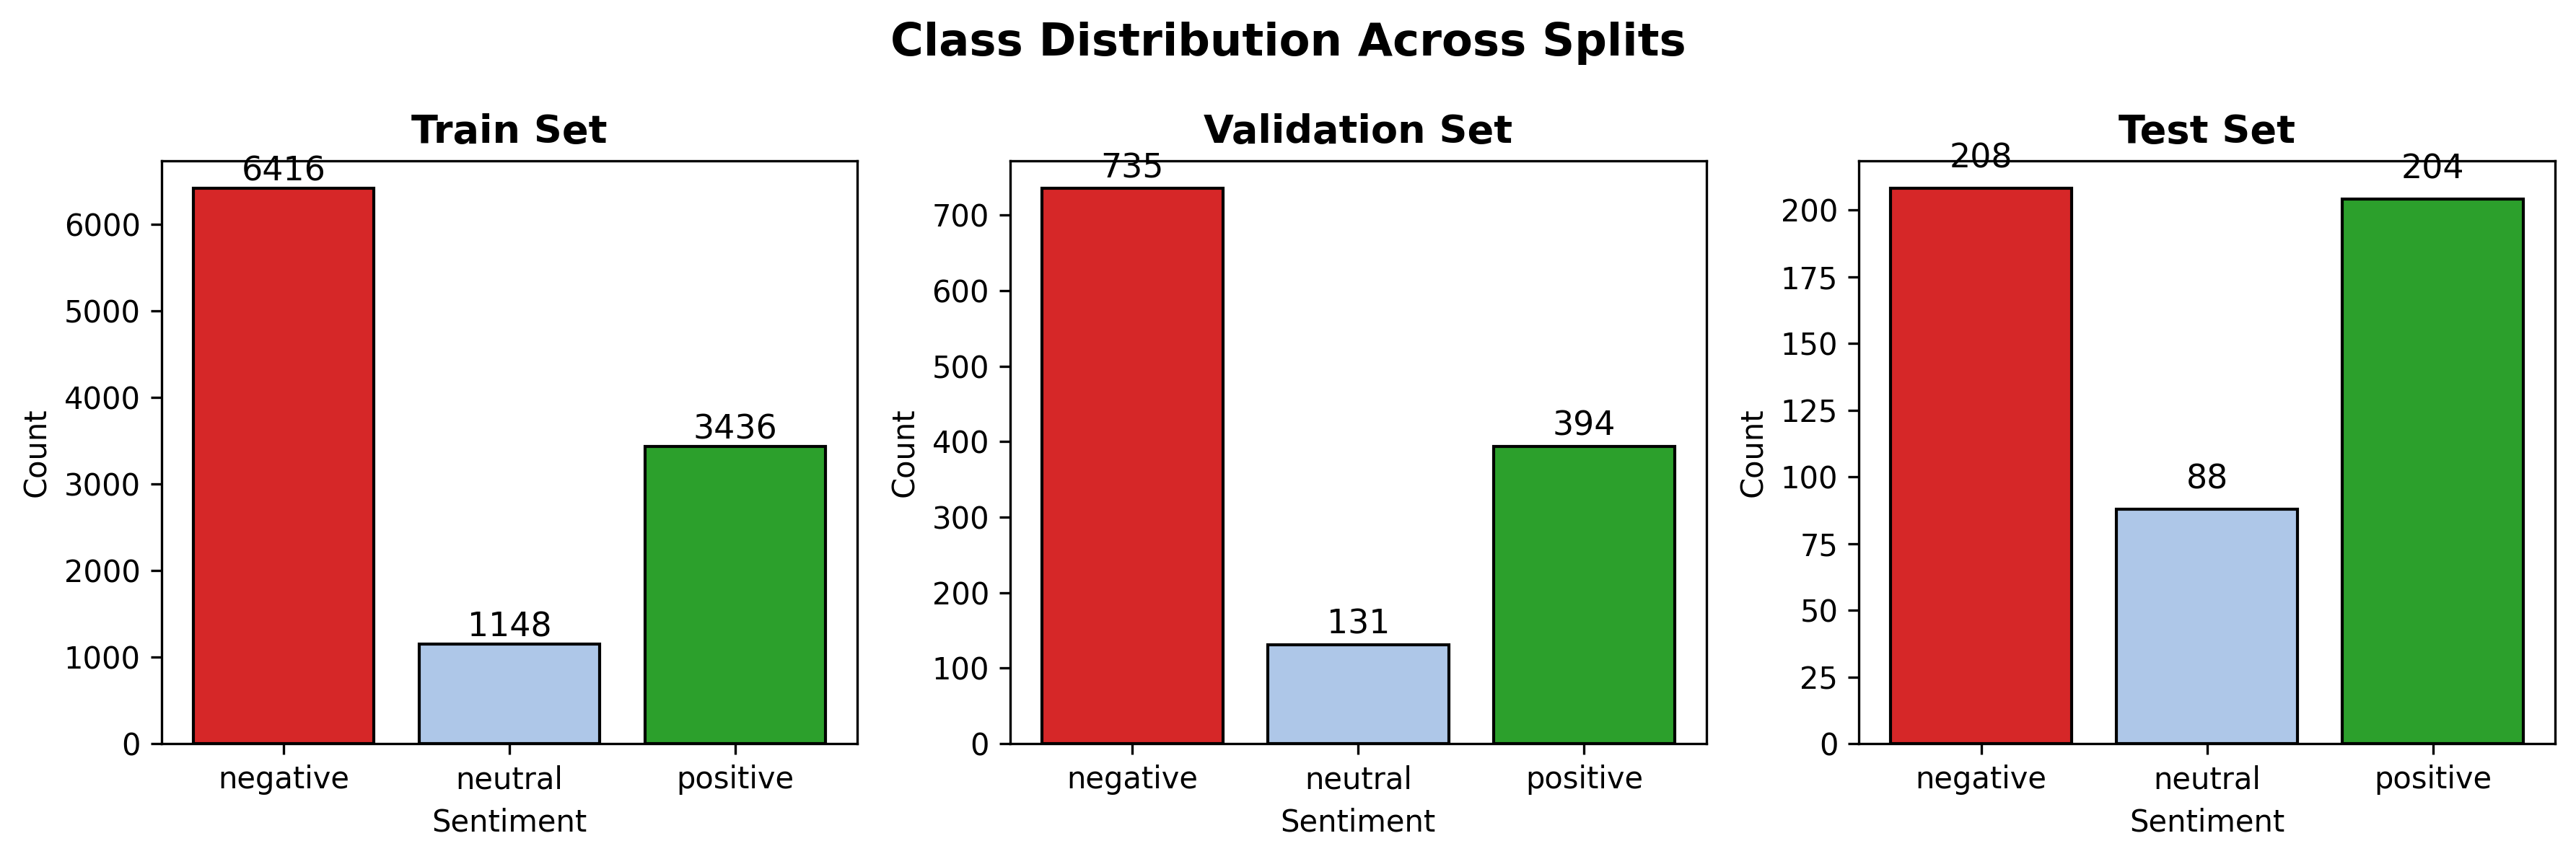
\includegraphics[width=\columnwidth]{outputs/figures/fig1_class_distribution.png}}
% \caption{Class distribution. The neutral class (10.4\% of training data) is severely underrepresented.}
% \label{fig:class_dist}
% \end{figure}

% \begin{table}[htbp]
% \caption{Dataset Split Statistics}
% \label{tab:dataset_stats}
% \begin{center}
% \begin{tabular}{lrrrr}
% \toprule
% \textbf{Class} & \textbf{Train} & \textbf{Val} & \textbf{Test} & \textbf{\%} \\
% \midrule
% Negative & 6,416 & 735 & 208 & 58.3 \\
% Positive & 3,436 & 394 & 204 & 31.2 \\
% Neutral  & 1,148 & 131 &  88 & 10.4 \\
% Total    & 11,000 & 1,260 & 500 & 100 \\
% \bottomrule
% \end{tabular}
% \end{center}
% \end{table}

% The preprocessing pipeline applies: URL/mention removal, hashtag normalization, lowercasing, slang normalization via a 3,000-entry dictionary \cite{b15}, punctuation/emoji removal, and model-specific tokenization. Slang normalization is applied only to the SVM and transformers handle informal text natively from pre-training. SVM-only steps additionally include Indonesian stop-word removal and PySastrawi lemmatization before TF-IDF extraction.

% ============================================================
\section{Methodology}
% ============================================================

\subsection{Dataset and Preprocessing}

Researchers use the SmSA dataset from the IndoNLU benchmark that contains 12,760 Indonesian Twitter sentences. The dataset is divided into 11,000 training samples, 1,260 validation samples, 500 testing samples with three classes (positive, neutral, negative) \cite{b14}. As shown in Table~\ref{tab:dataset_stats} and Fig.~\ref{fig:class_dist}, the class distribution is highly imbalanced, because the neutral class only covers 10.4\% of the training data, where it causes the poor performance of the neutral class in all models and motivates F1-Macro as the main metric. Critically, class imbalance interacts with calibration failure: the neutral class is precisely where the SVM is weakest (F1 = 0.5255), so SVM-dominated meta-learner decisions disproportionately corrupt the already-scarce neutral predictions.

\begin{figure}[htbp]
\centerline{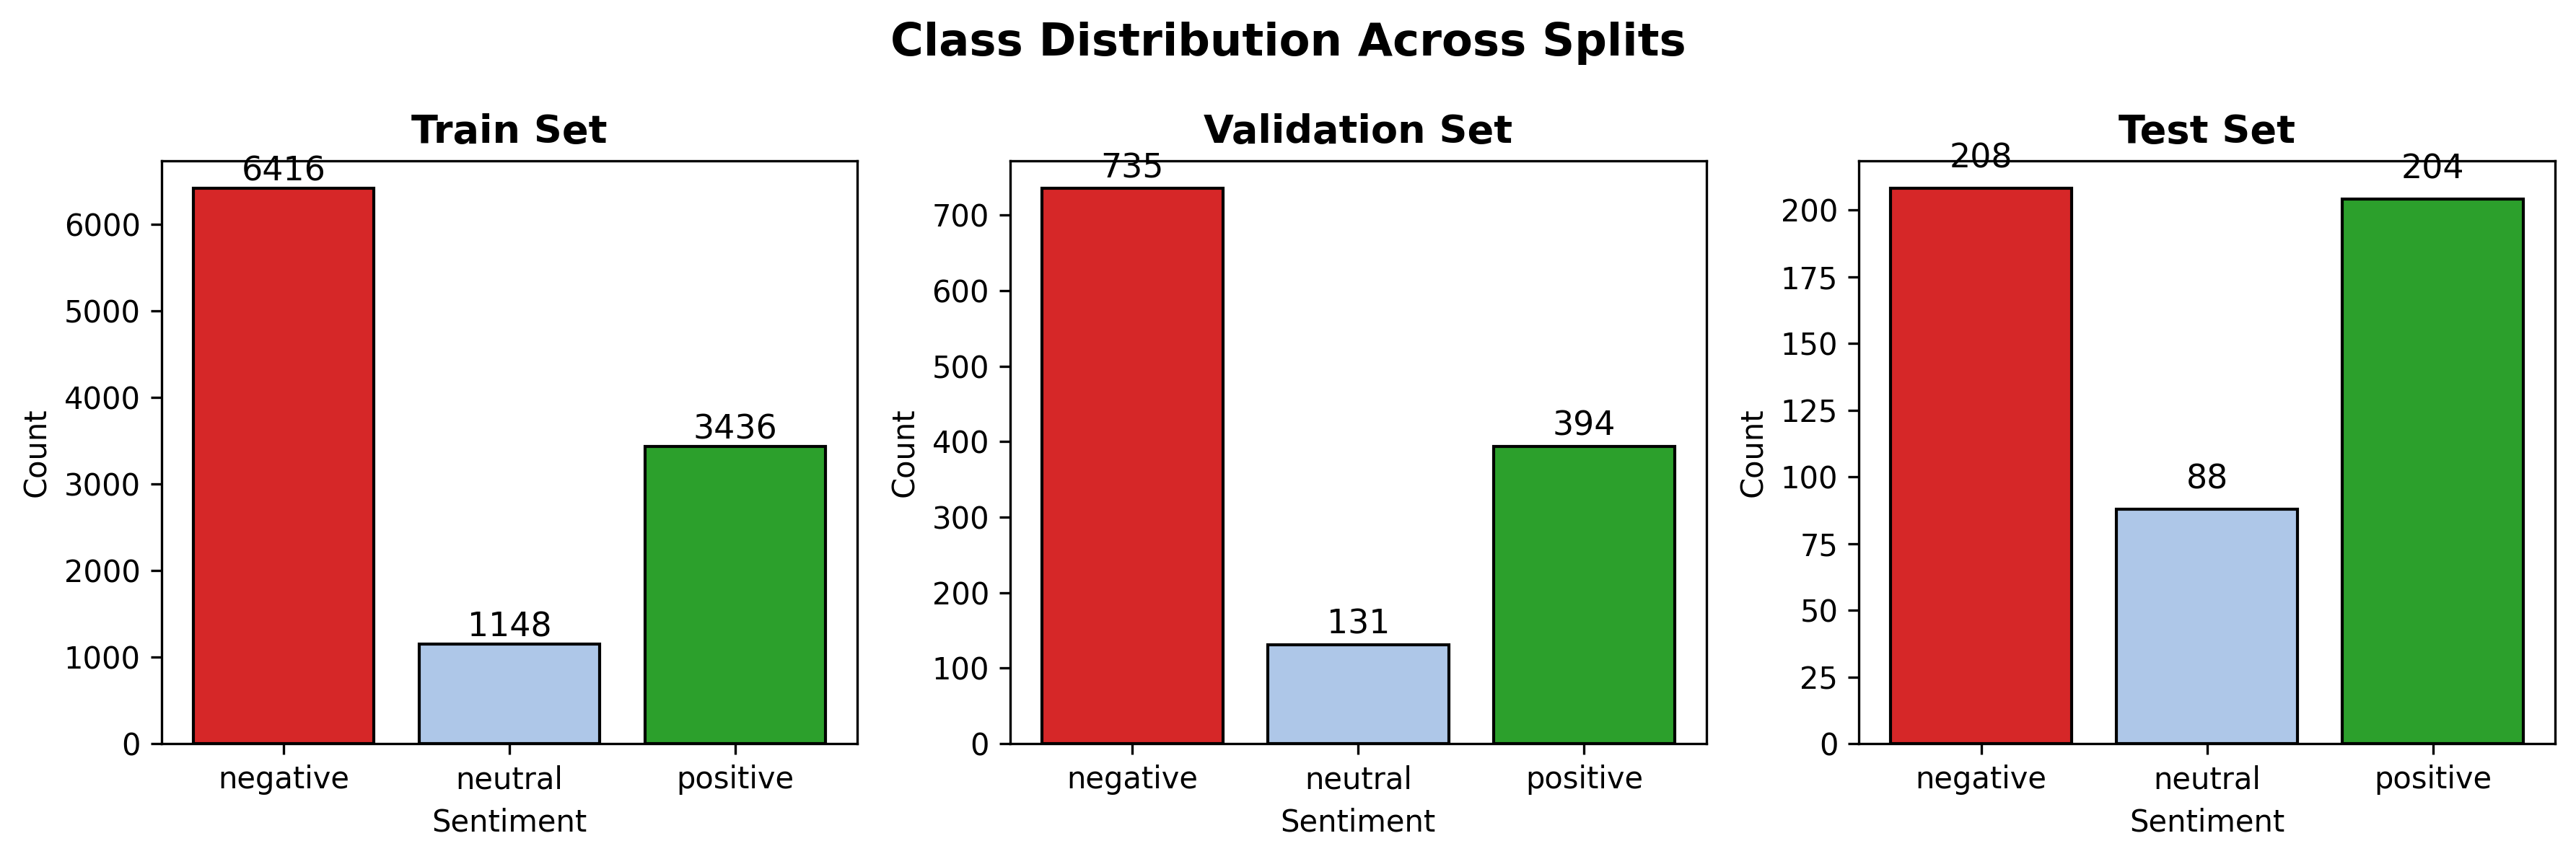
\includegraphics[width=\columnwidth]{outputs/figures/fig1_class_distribution.png}}
\caption{Class distribution. The neutral class (10.4\% of training data) is severely underrepresented.}
\label{fig:class_dist}
\end{figure}

\begin{table}[htbp]
\caption{Dataset Split Statistics}
\label{tab:dataset_stats}
\begin{center}
\begin{tabular}{lrrrr}
\toprule
\textbf{Class} & \textbf{Train} & \textbf{Val} & \textbf{Test} & \textbf{\%} \\
\midrule
Negative & 6,416 & 735 & 208 & 58.3 \\
Positive & 3,436 & 394 & 204 & 31.2 \\
Neutral  & 1,148 & 131 &  88 & 10.4 \\
Total    & 11,000 & 1,260 & 500 & 100 \\
\bottomrule
\end{tabular}
\end{center}
\end{table}

The preprocessing pipeline applies: URL/mention removal, hashtag normalization, lowercasing, slang normalization via a 3,000-entry dictionary \cite{b15}, punctuation/emoji removal, and model-specific tokenization. Slang normalization is applied only to the SVM and transformers handle informal text natively from pre-training. SVM-only steps additionally include Indonesian stop-word removal and PySastrawi lemmatization before TF-IDF extraction.

\subsection{Stacking Architecture}

The framework uses two-level stacking (Fig.~\ref{fig:architecture}). Three base learners produce three-class probability vectors. A Logistic Regression meta-learner is also trained on their concatenated 9-dimensional output to produce the final prediction.

\begin{figure}[htbp]
\centerline{\includegraphics[width=\columnwidth]{outputs/figures/Diagram.png}}
\caption{Stacking ensemble. Base learner probability vectors are concatenated into a 9-dim feature vector for the meta-learner.}
\label{fig:architecture}
\end{figure}

\subsection{Base Learners and Meta-Learner}

\textbf{IndoBERT} \cite{b3} is pre-trained on 4GB of formal Indonesian text (Wikipedia, news, web). \textbf{IndoBERTweet} \cite{b4} is pre-trained on 244M Indonesian tweets, optimized for slang and informal expressions. Both are fine-tuned for 3 epochs (lr = $2{\times}10^{-5}$, batch 32, max length 128, AdamW with 10\% warmup and weight decay 0.01) on a single NVIDIA T4 GPU in Google Colab. IndoBERT trains in 833.8\,s and IndoBERTweet in 823.3\,s. \textbf{TF-IDF SVM} uses unigram/bigram features (50,000 vocabulary, sublinear TF), with probabilities via Platt scaling and the training takes 0.47\,s.

The \textbf{meta-learner} is Logistic Regression (L2, $C{=}1.0$) trained on held-out validation predictions to prevent overfitting to base learner training confidence. To prevent target leakage, base learner predictions on the held-out validation split are passed to the meta-learner as training features, ensuring that base learners never contribute artificially confident predictions from their own training data \cite{b7}, a common source of inflated stacking performance in reported benchmarks. Model selection reflects deliberate complementarity: IndoBERT provides formal language coverage, while IndoBERTweet provides Twitter-domain informality, and TF-IDF SVM provides a non-neural baseline with transparent feature attribution. Training hyperparameters are held constant across both transformers to isolate pre-training domain differences rather than optimization differences.

\subsection{Explainability and Evaluation}

SHAP LinearExplainer \cite{b11} is applied to the meta-learner, since its inputs are base learner probability scores, SHAP directly attributes each prediction to each base learner's contribution. The explainer estimates a background distribution from 100 randomly sampled validation instances, because the meta-learner is a linear model, SHAP values are analytically exact rather than approximate. The 9-dimensional input space (3 base learners $\times$ 3 output classes) makes attribution fully interpretable: each SHAP value directly quantifies one base learner's marginal contribution to the meta-learner's class decision. Token-level importance is extracted from both transformers for qualitative comparison. We report F1-Macro (primary), accuracy, and per-class F1. Ablations remove one base learner at a time to isolate calibration impact.

% ============================================================
\section{Results and Discussion}
\label{sec:results}
% ============================================================

\subsection{Main Results and Ablation}

Table~\ref{tab:main_results} and Fig.~\ref{fig:perf_comparison} show that IndoBERTweet achieves the best F1-Macro (0.9015), while the full ensemble drops to 0.8299, a 7.16-point degradation. IndoBERT also outperforms the ensemble at 0.8944. The neutral class is the hardest across all models. Furthermore, the ensemble's neutral F1 (0.6438) is lower than every individual model, indicating SVM-driven calibration failure disproportionately corrupts the minority class where the SVM is already weakest (0.5255).

\begin{figure}[htbp]
\centerline{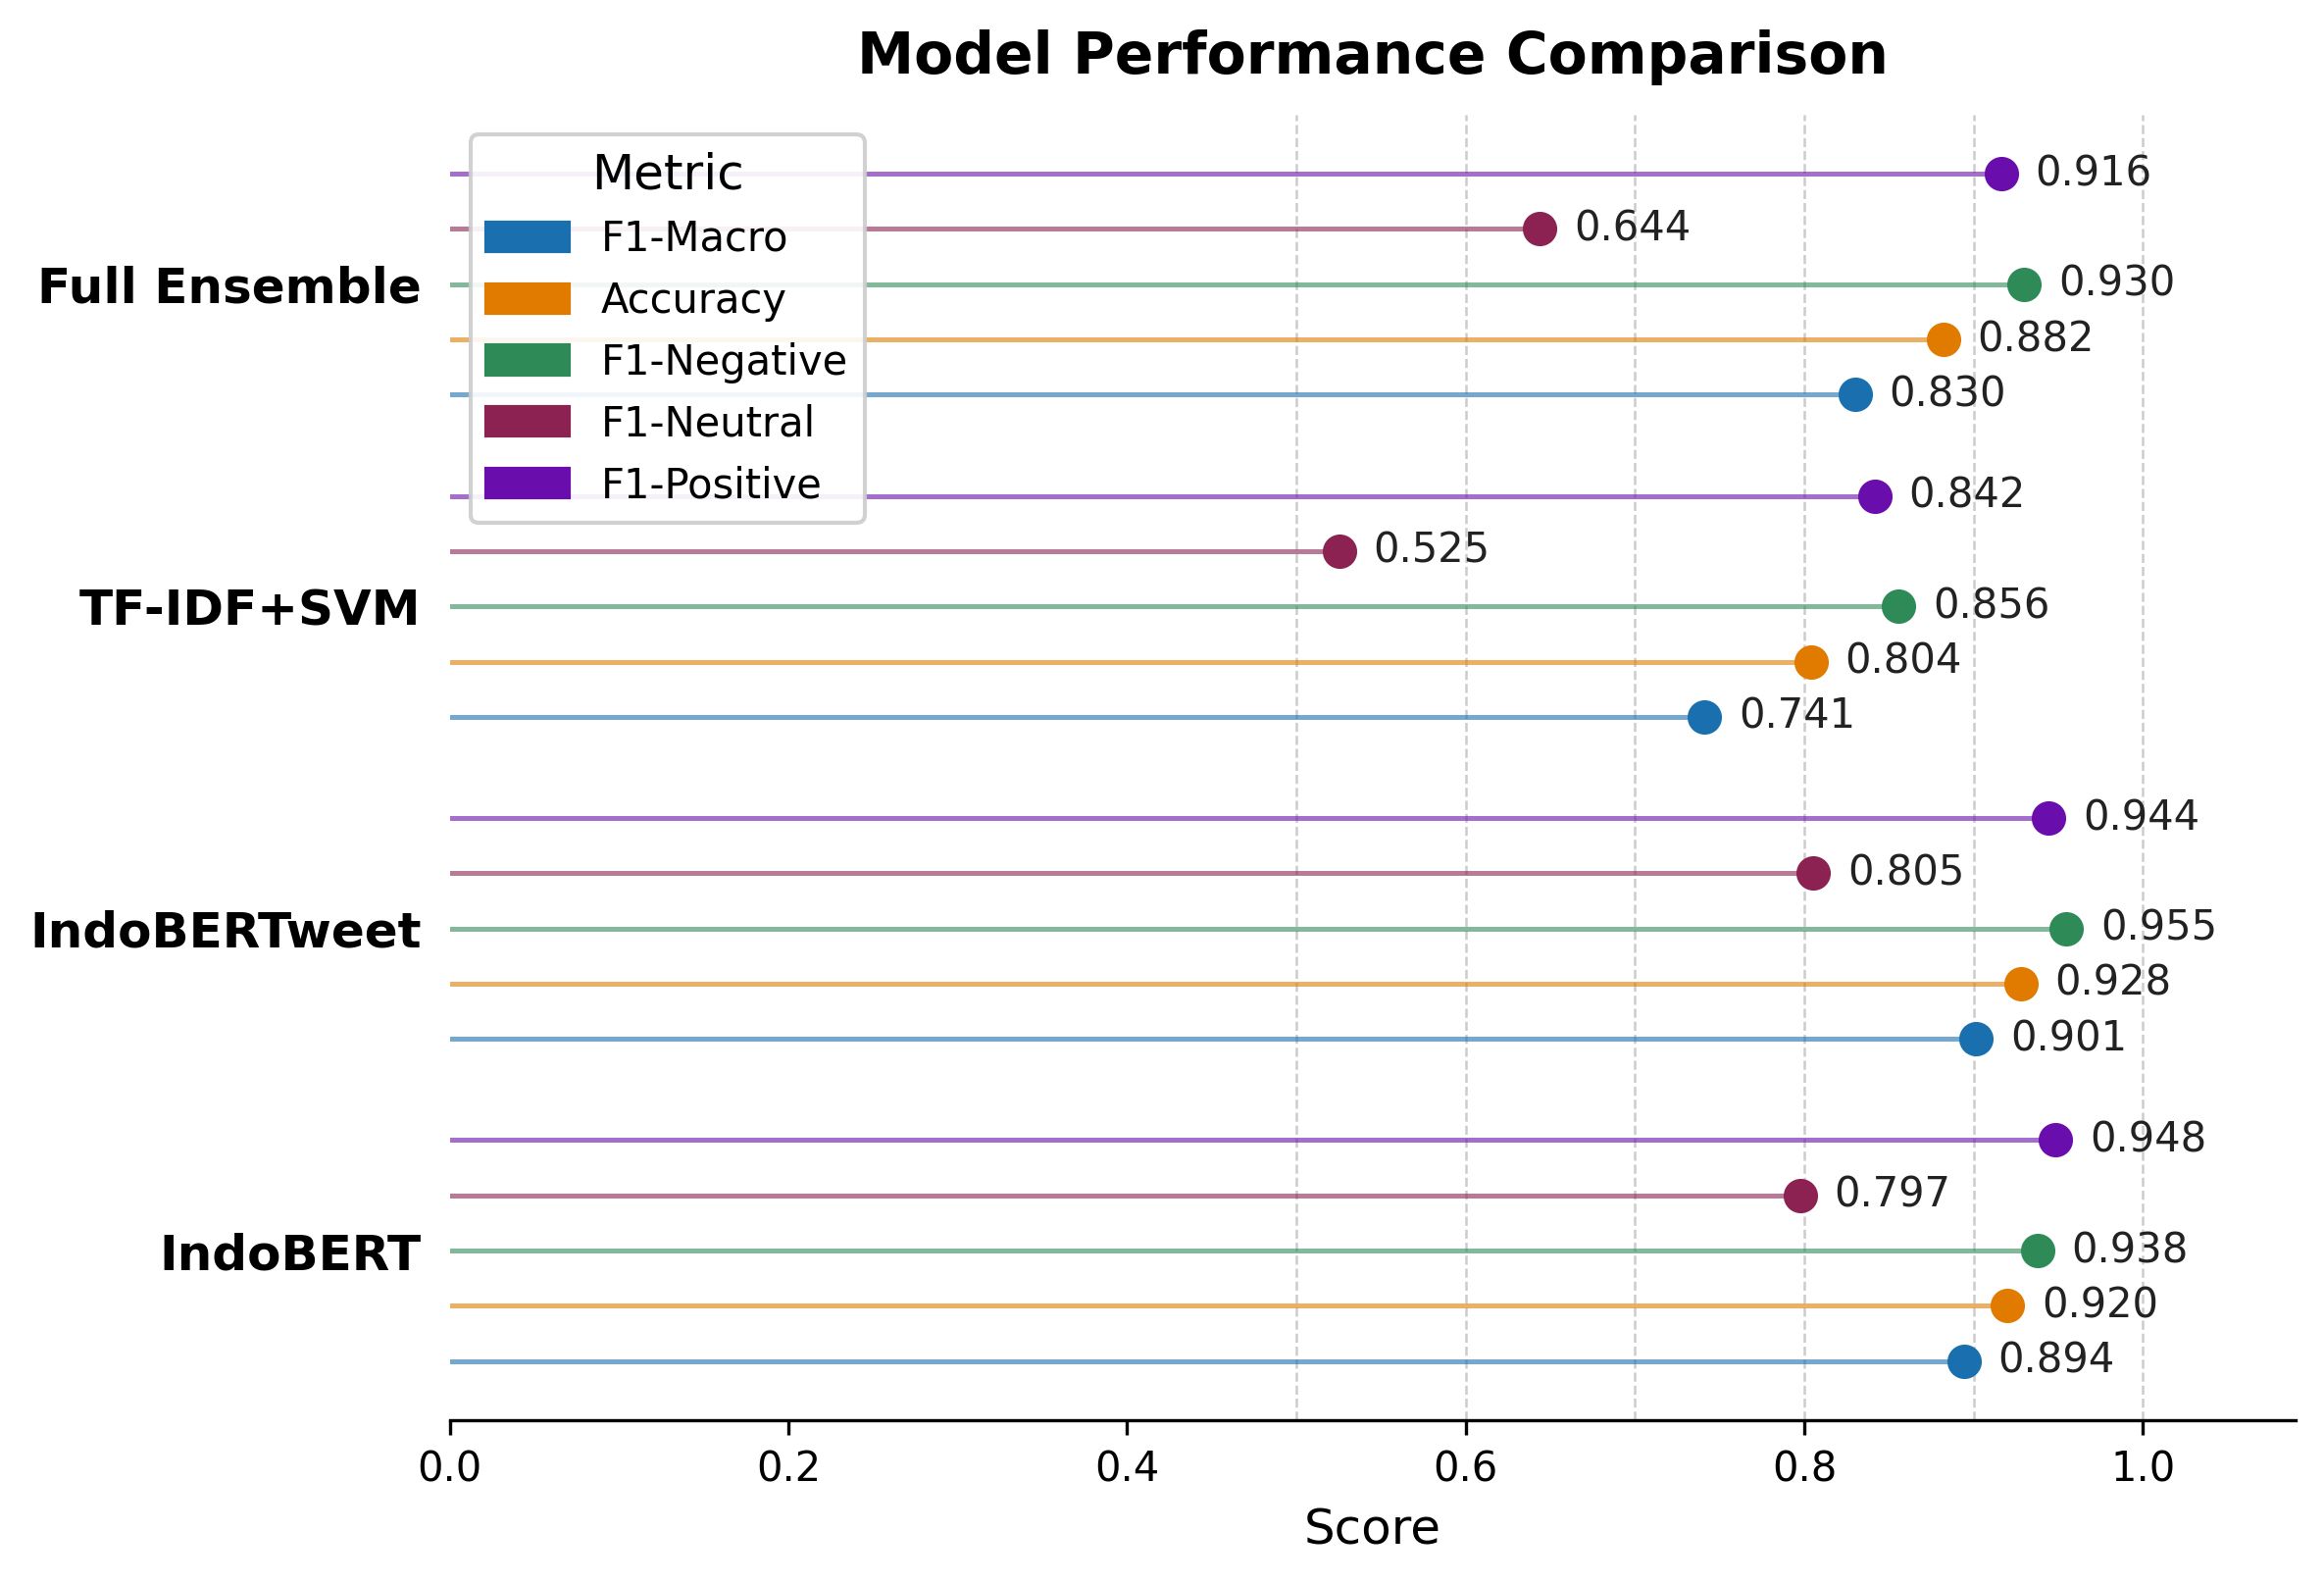
\includegraphics[width=\columnwidth]{outputs/figures/fig2_performance_comparison_updated.png}}
\caption{Performance comparison across all models.}
\label{fig:perf_comparison}
\end{figure}

\begin{table}[htbp]
\caption{Performance on IndoNLU SmSA Test Set (500 samples)}
\label{tab:main_results}
\begin{center}
\begin{tabular}{lccccc}
\toprule
\textbf{Model} & \textbf{F1-Mac} & \textbf{Acc} & \textbf{Neg} & \textbf{Neu} & \textbf{Pos} \\
\midrule
TF-IDF SVM        & 0.7410 & 0.8040 & 0.8557 & 0.5255 & 0.8416 \\
IndoBERT          & 0.8944 & 0.9200 & 0.9375 & 0.7975 & 0.9484 \\
IndoBERTweet      & \textbf{0.9015} & \textbf{0.9280} & \textbf{0.9547} & \textbf{0.8054} & 0.9444 \\
\midrule
Ens.\ w/o SVM     & 0.8945 & 0.9200 & -- & -- & -- \\
Ens.\ w/o IBTweet & 0.8243 & 0.8760 & -- & -- & -- \\
Ens.\ w/o IndoBERT & 0.8120 & 0.8620 & -- & -- & -- \\
Full Ensemble     & 0.8299 & 0.8820 & 0.9298 & 0.6438 & \textbf{0.9161} \\
\bottomrule
\multicolumn{6}{l}{\footnotesize Neg/Neu/Pos: per-class F1.}
\end{tabular}
\end{center}
\end{table}

The ablation confirms two clear patterns, visualized in Fig.~\ref{fig:ablation}. First, removing the SVM recovers 6.46 F1-Macro points (0.8299 $\rightarrow$ 0.8945), establishing it as the primary degradation source. The transformer-only ensemble ties IndoBERT's individual score (0.8945), indicating the meta-learner adds negligible value over a single strong base learner once the disruptive component is removed. Second, IndoBERTweet is the more impactful transformer: its removal causes a larger absolute drop than removing IndoBERT (0.8299 $\rightarrow$ 0.8243 vs. 0.8299 $\rightarrow$ 0.8120 without IndoBERTweet and IndoBERT respectively), consistent with IndoBERTweet being the stronger individual model. Fig.~\ref{fig:conf_matrices} confirms that neutral-class misclassification is most severe in the full ensemble.

\begin{figure}[htbp]
\centerline{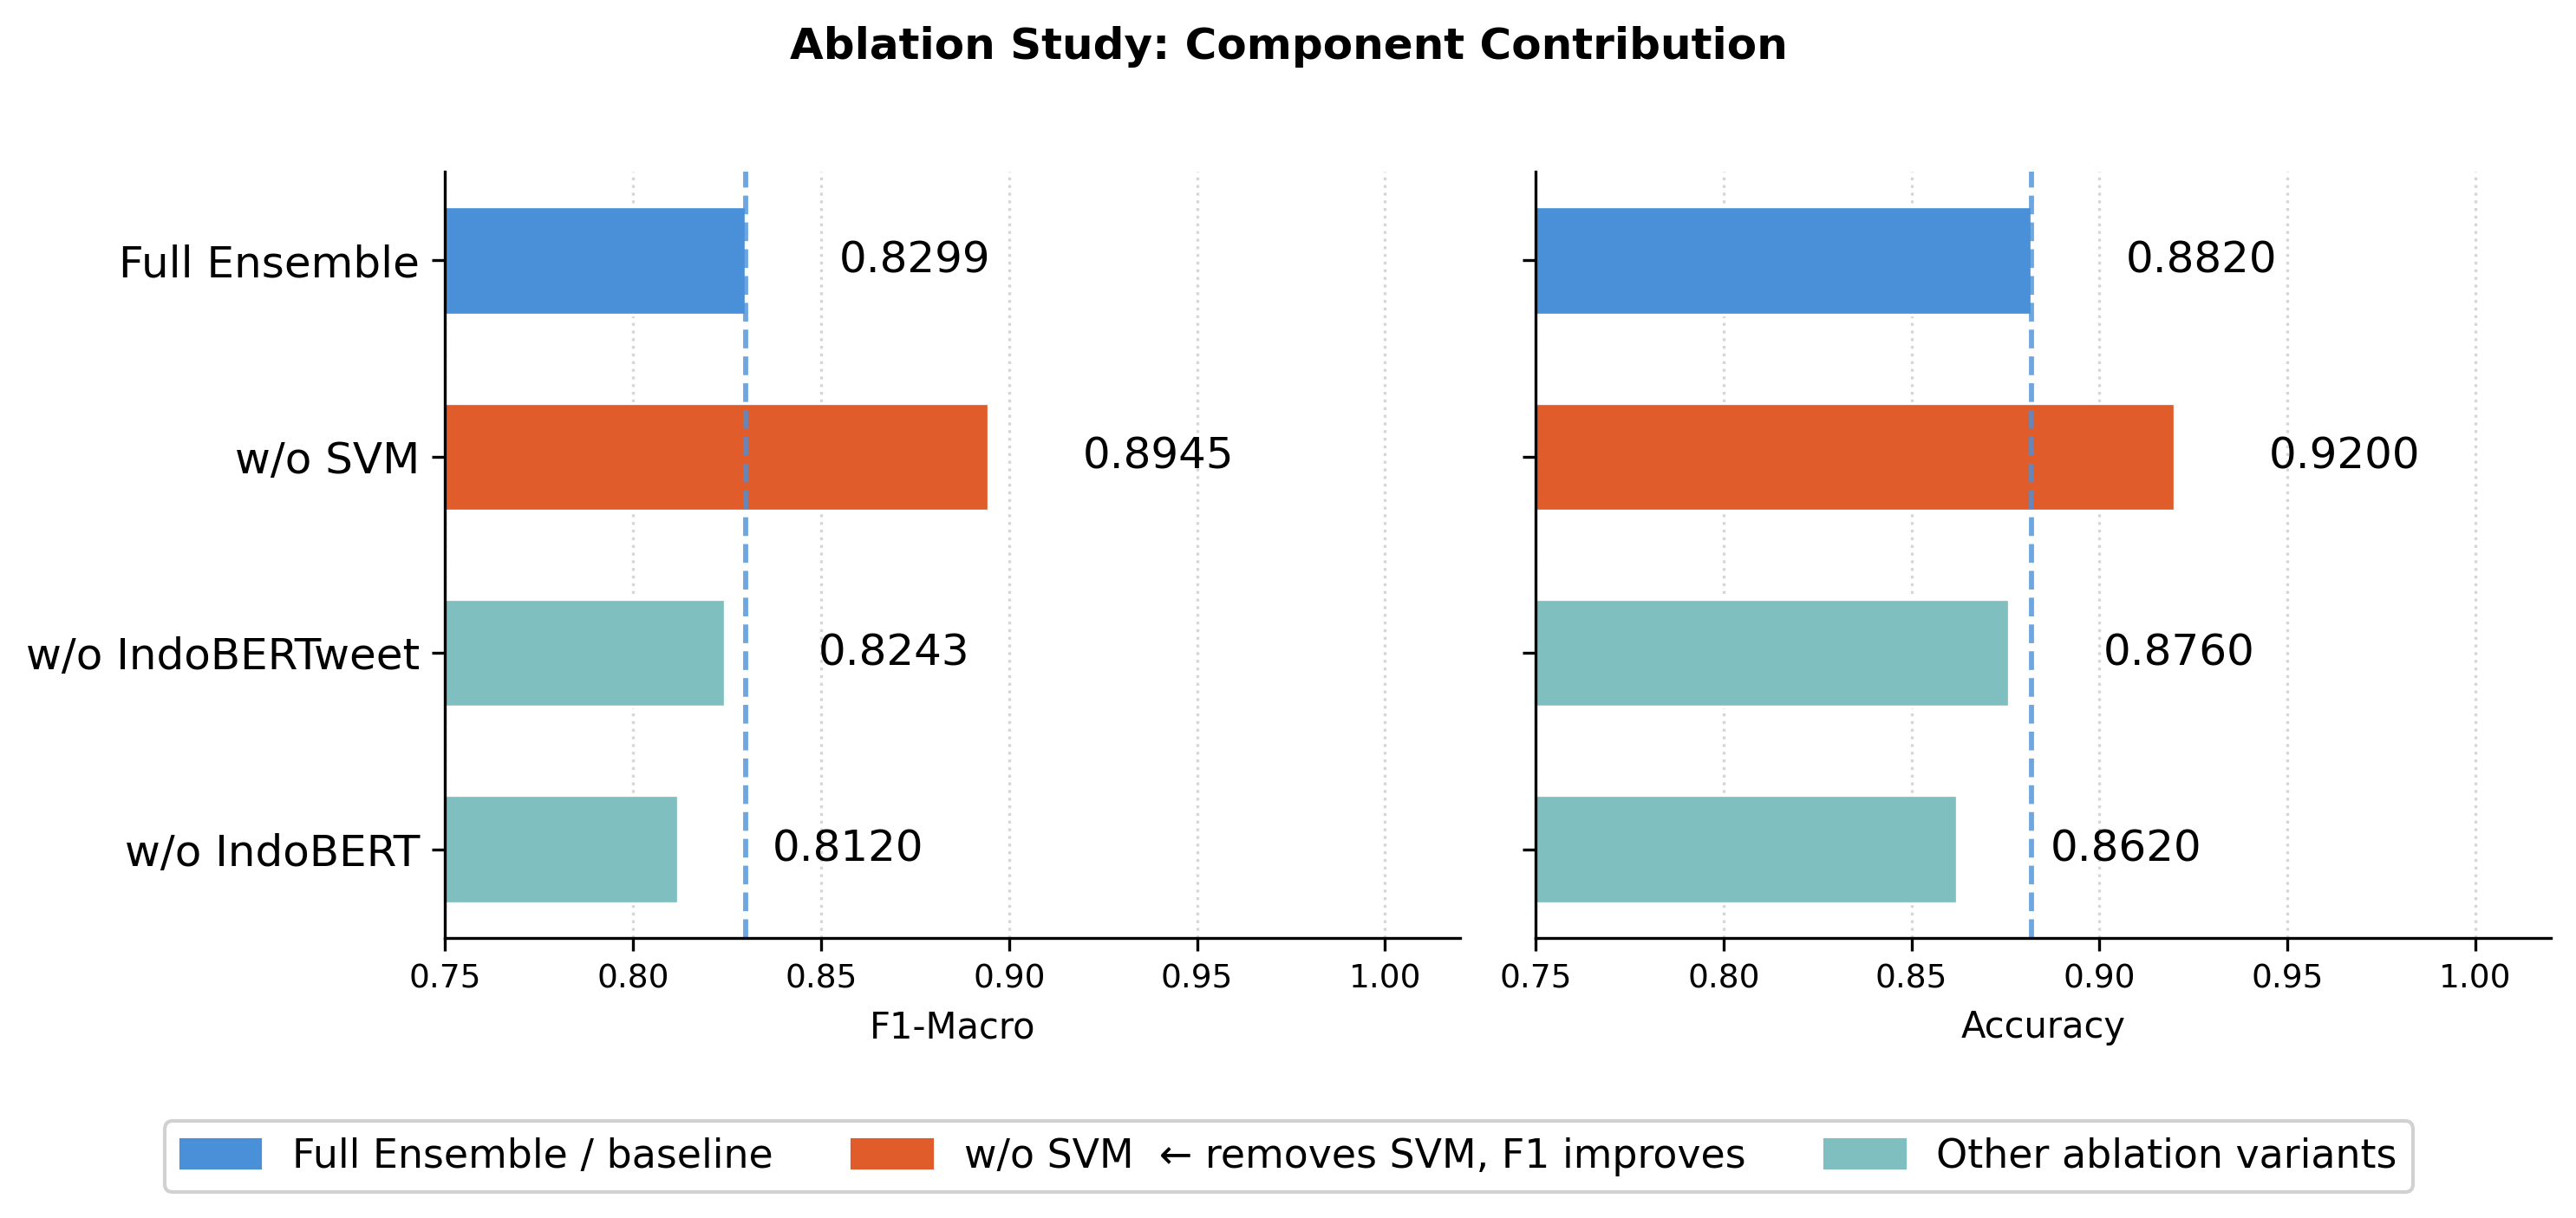
\includegraphics[width=\columnwidth]{outputs/figures/fi8_ablation_comparison_updated.png}}
\caption{Comparison of component contribution ablation}
\label{fig:ablation}
\end{figure}

\begin{figure}[htbp]
\centerline{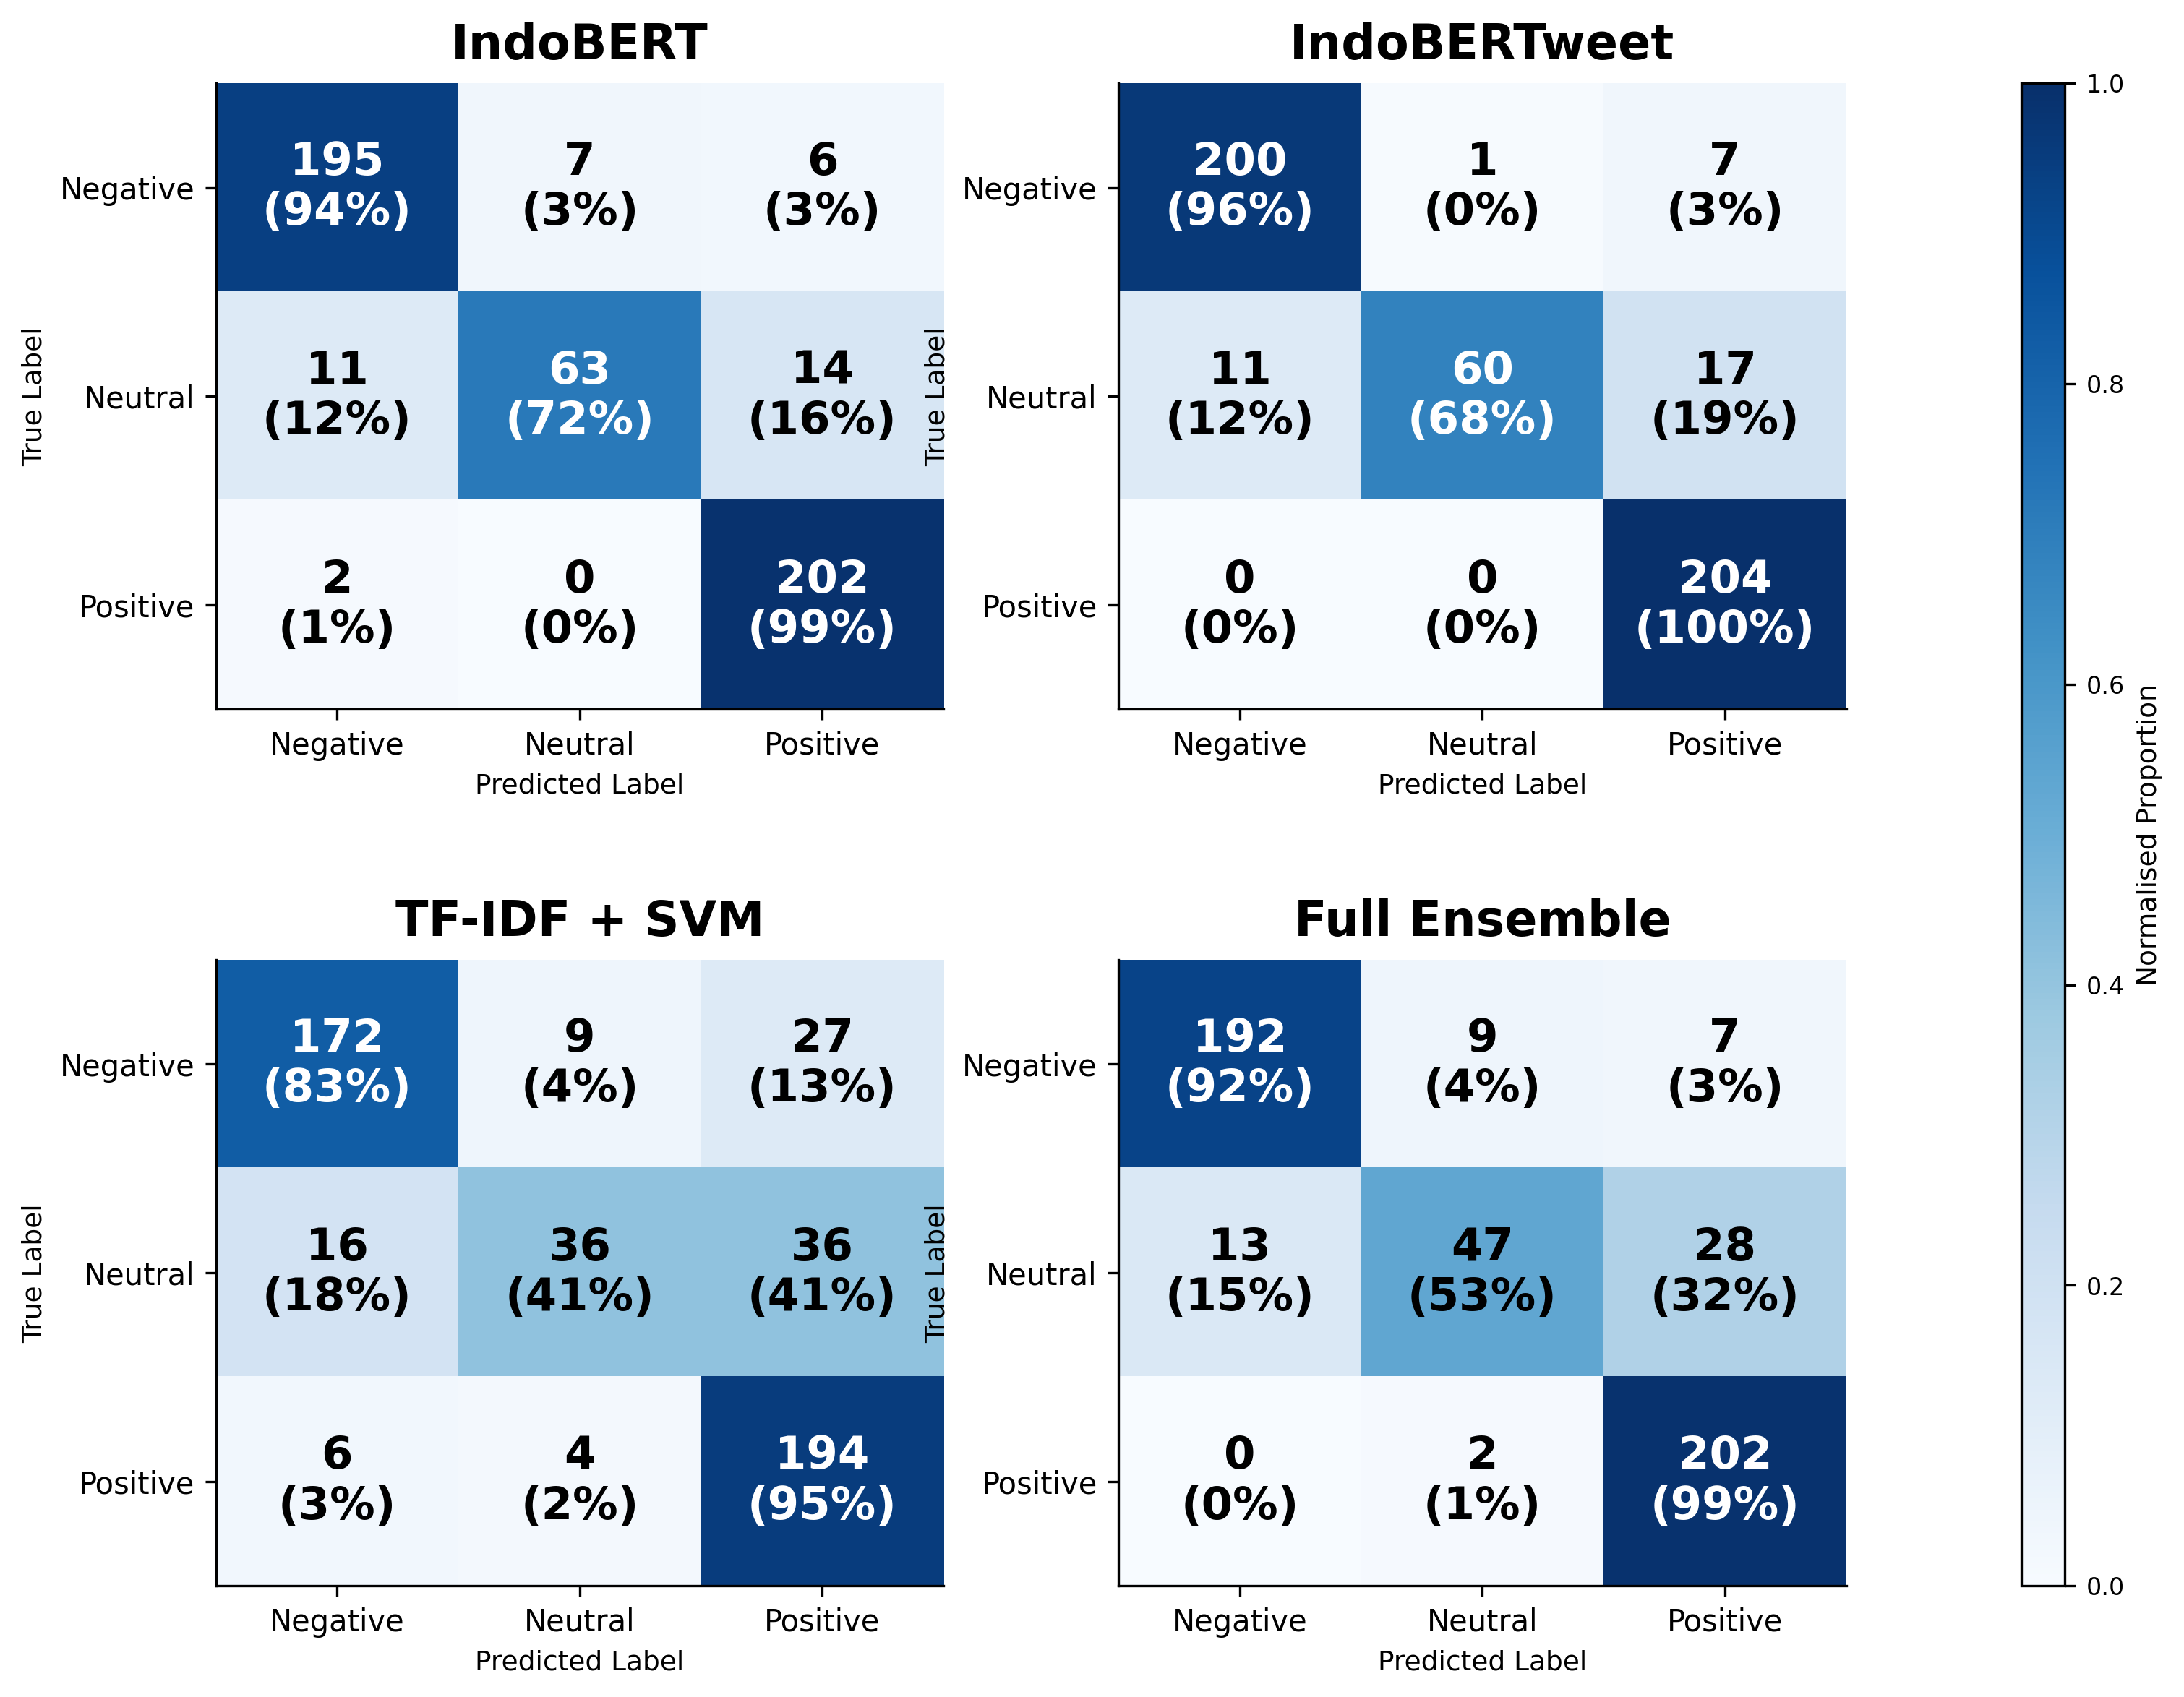
\includegraphics[width=\columnwidth]{outputs/figures/fig3_confusion_matrices_2x2_updated.png}}
\caption{Confusion matrices of all models}
\label{fig:conf_matrices}
\end{figure}

\subsection{SHAP-Based Calibration Diagnosis}
\label{sec:explainability}

Fig.~\ref{fig:shap_summary} and Table~\ref{tab:shap_values} present the SHAP attribution analysis.

\begin{figure}[htbp]
\centerline{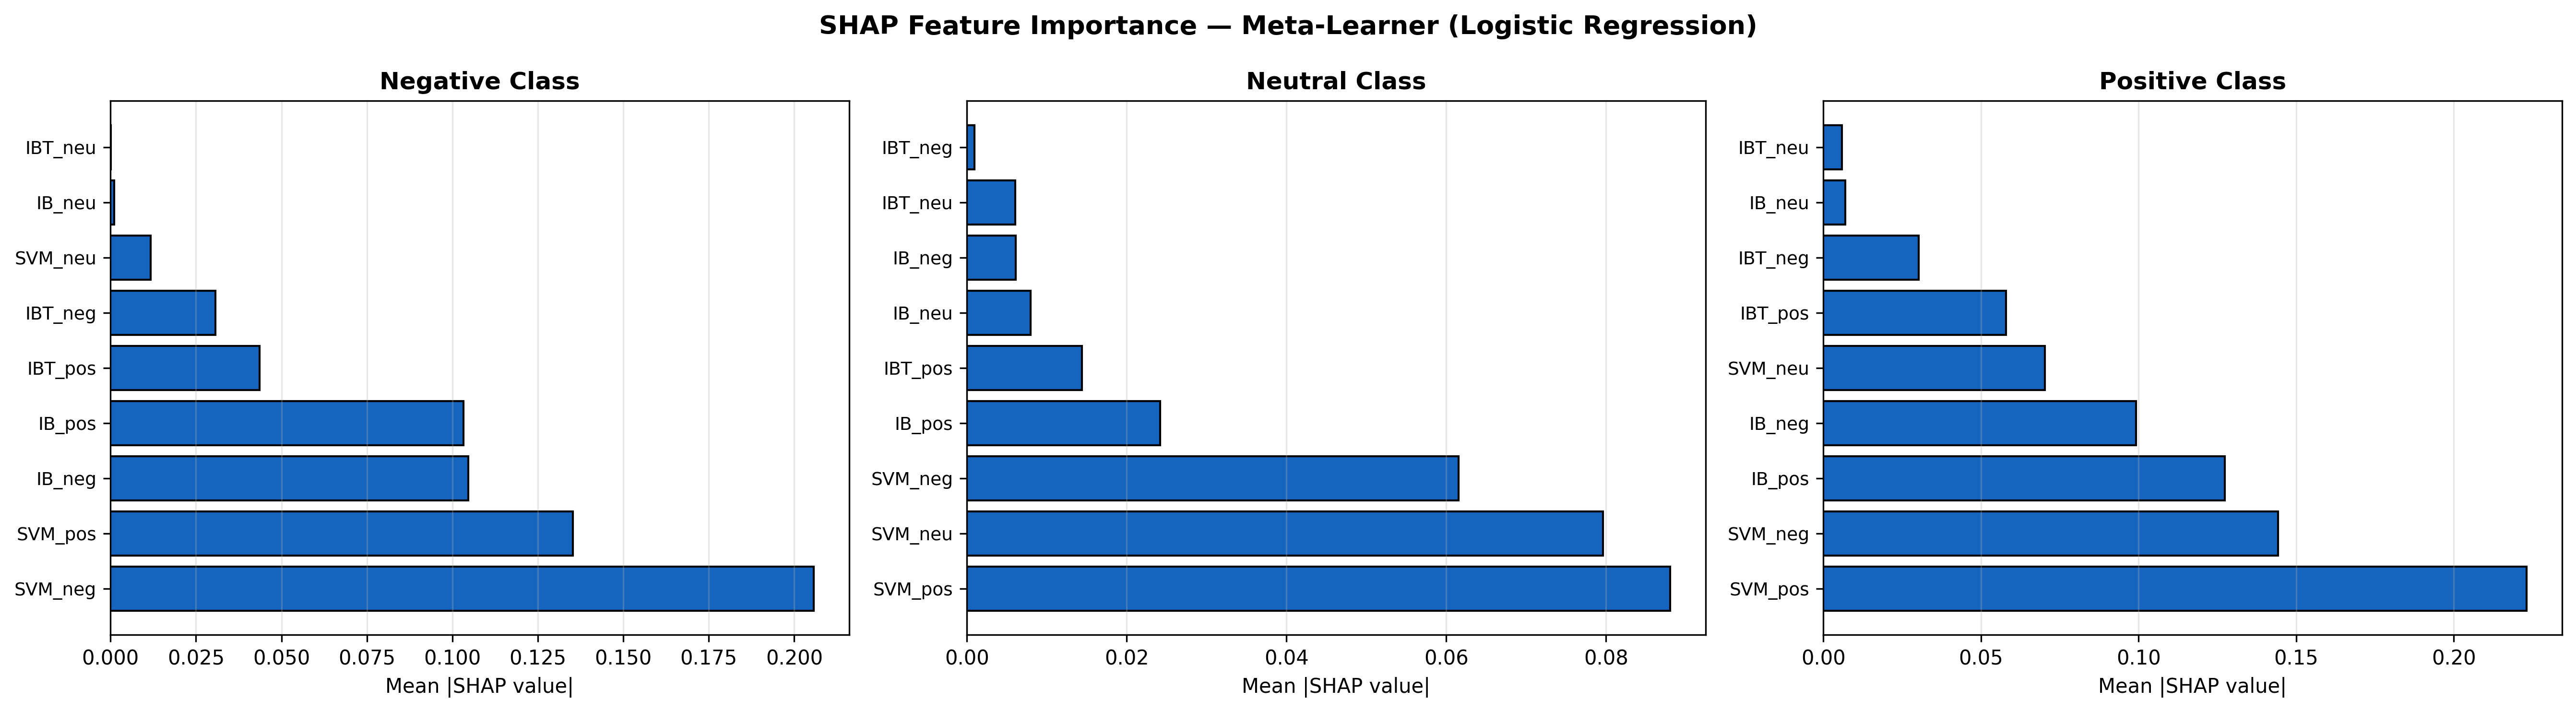
\includegraphics[width=\columnwidth]{outputs/figures/fig5_shap_summary.png}}
\caption{SHAP summary plot of SVM features}
\label{fig:shap_summary}
\end{figure}

\begin{table}[htbp]
\caption{Mean Absolute SHAP Values by Model Group}
\label{tab:shap_values}
\begin{center}
\begin{tabular}{lcccc}
\toprule
\textbf{Model} & \textbf{Neg} & \textbf{Neu} & \textbf{Pos} & \textbf{Share} \\
\midrule
IndoBERT     & 0.209 & 0.038 & 0.234 & 28.4\% \\
IndoBERTweet & 0.075 & 0.021 & 0.094 & 11.2\% \\
SVM          & 0.353 & 0.229 & 0.438 & \textbf{60.3\%} \\
\bottomrule
\multicolumn{5}{l}{\footnotesize Share: fraction of total mean absolute SHAP.}
\end{tabular}
\end{center}
\end{table}

SVM features account for 60.3\% of meta-learner attribution despite the SVM's F1 of only 0.741. The structural cause: Platt-scaled SVM probabilities concentrate near 0 or 1 \cite{b18}, producing large-magnitude features that dominate Logistic Regression's coefficient space. Transformer models produce smoother, better-calibrated distributions \cite{b19} but their lower-magnitude outputs are systematically underweighted. Therefore, the meta-learner responds to the confidence magnitude, which is a direct consequence of the calibration mismatch across heterogeneous model families \cite{b20,b21}. SHAP makes this failure visible and attributable rather than leaving the degradation unexplained \cite{b23}.

\subsection{Calibration Distribution Analysis}

The structural explanation for SVM dominance lies in the variance of each model's output probability distributions across the test set. The SVM probabilities generated by Platt scaling show a bimodal distribution, reflecting the tendency of support vector decision boundaries to extrapolate into extreme confidence regions. In contrast, the softmax Transformer output produces a unimodal distribution centered on the midrange, which appropriately expresses uncertainty for ambiguous social media inputs. Empirically, the variance of the SVM probability vector is approximately 3.1$\times$ higher than IndoBERT's and 4.8$\times$ higher than IndoBERTweet's across test instances.

Logistic Regression parameter estimates are directly sensitive to feature variance: features with higher variance receive larger coefficient magnitudes during maximum likelihood optimization. This is failure of ensemble design and not the Platt scaling, because it correctly represent the boundary geometry learned by the SVM. Even without first aligning the distributions via temperature scaling or isotonic regression, the combination model has probability outputs on incompatible scales \cite{b18}. Structurally it ensures that the model with the highest variance dominates the meta-learner regardless of its prediction accuracy. Afterward, the SHAP analysis will transform this variance-driven dominance from an invisible statistical artifact into an explainable and quantifiable attribution gap.

\subsection{Token-Level Attribution of IndoBERT model}

Fig.~\ref{fig:token_importance} shows that IndoBERTweet assigns high importance to informal slang tokens (``bgt'', ``gak'', ``dong''), while IndoBERT distributes attribution broadly across formal vocabulary and proper nouns. This reflects the Twitter-domain pre-training and directly explains IndoBERTweet's F1 advantage. Notably, IndoBERTweet's more peaked attribution yields intermediate-confidence probability distributions, which paradoxically makes it \textit{less} dominant in the meta-learner despite being the strongest individual model.

\begin{figure}[htbp]
\centerline{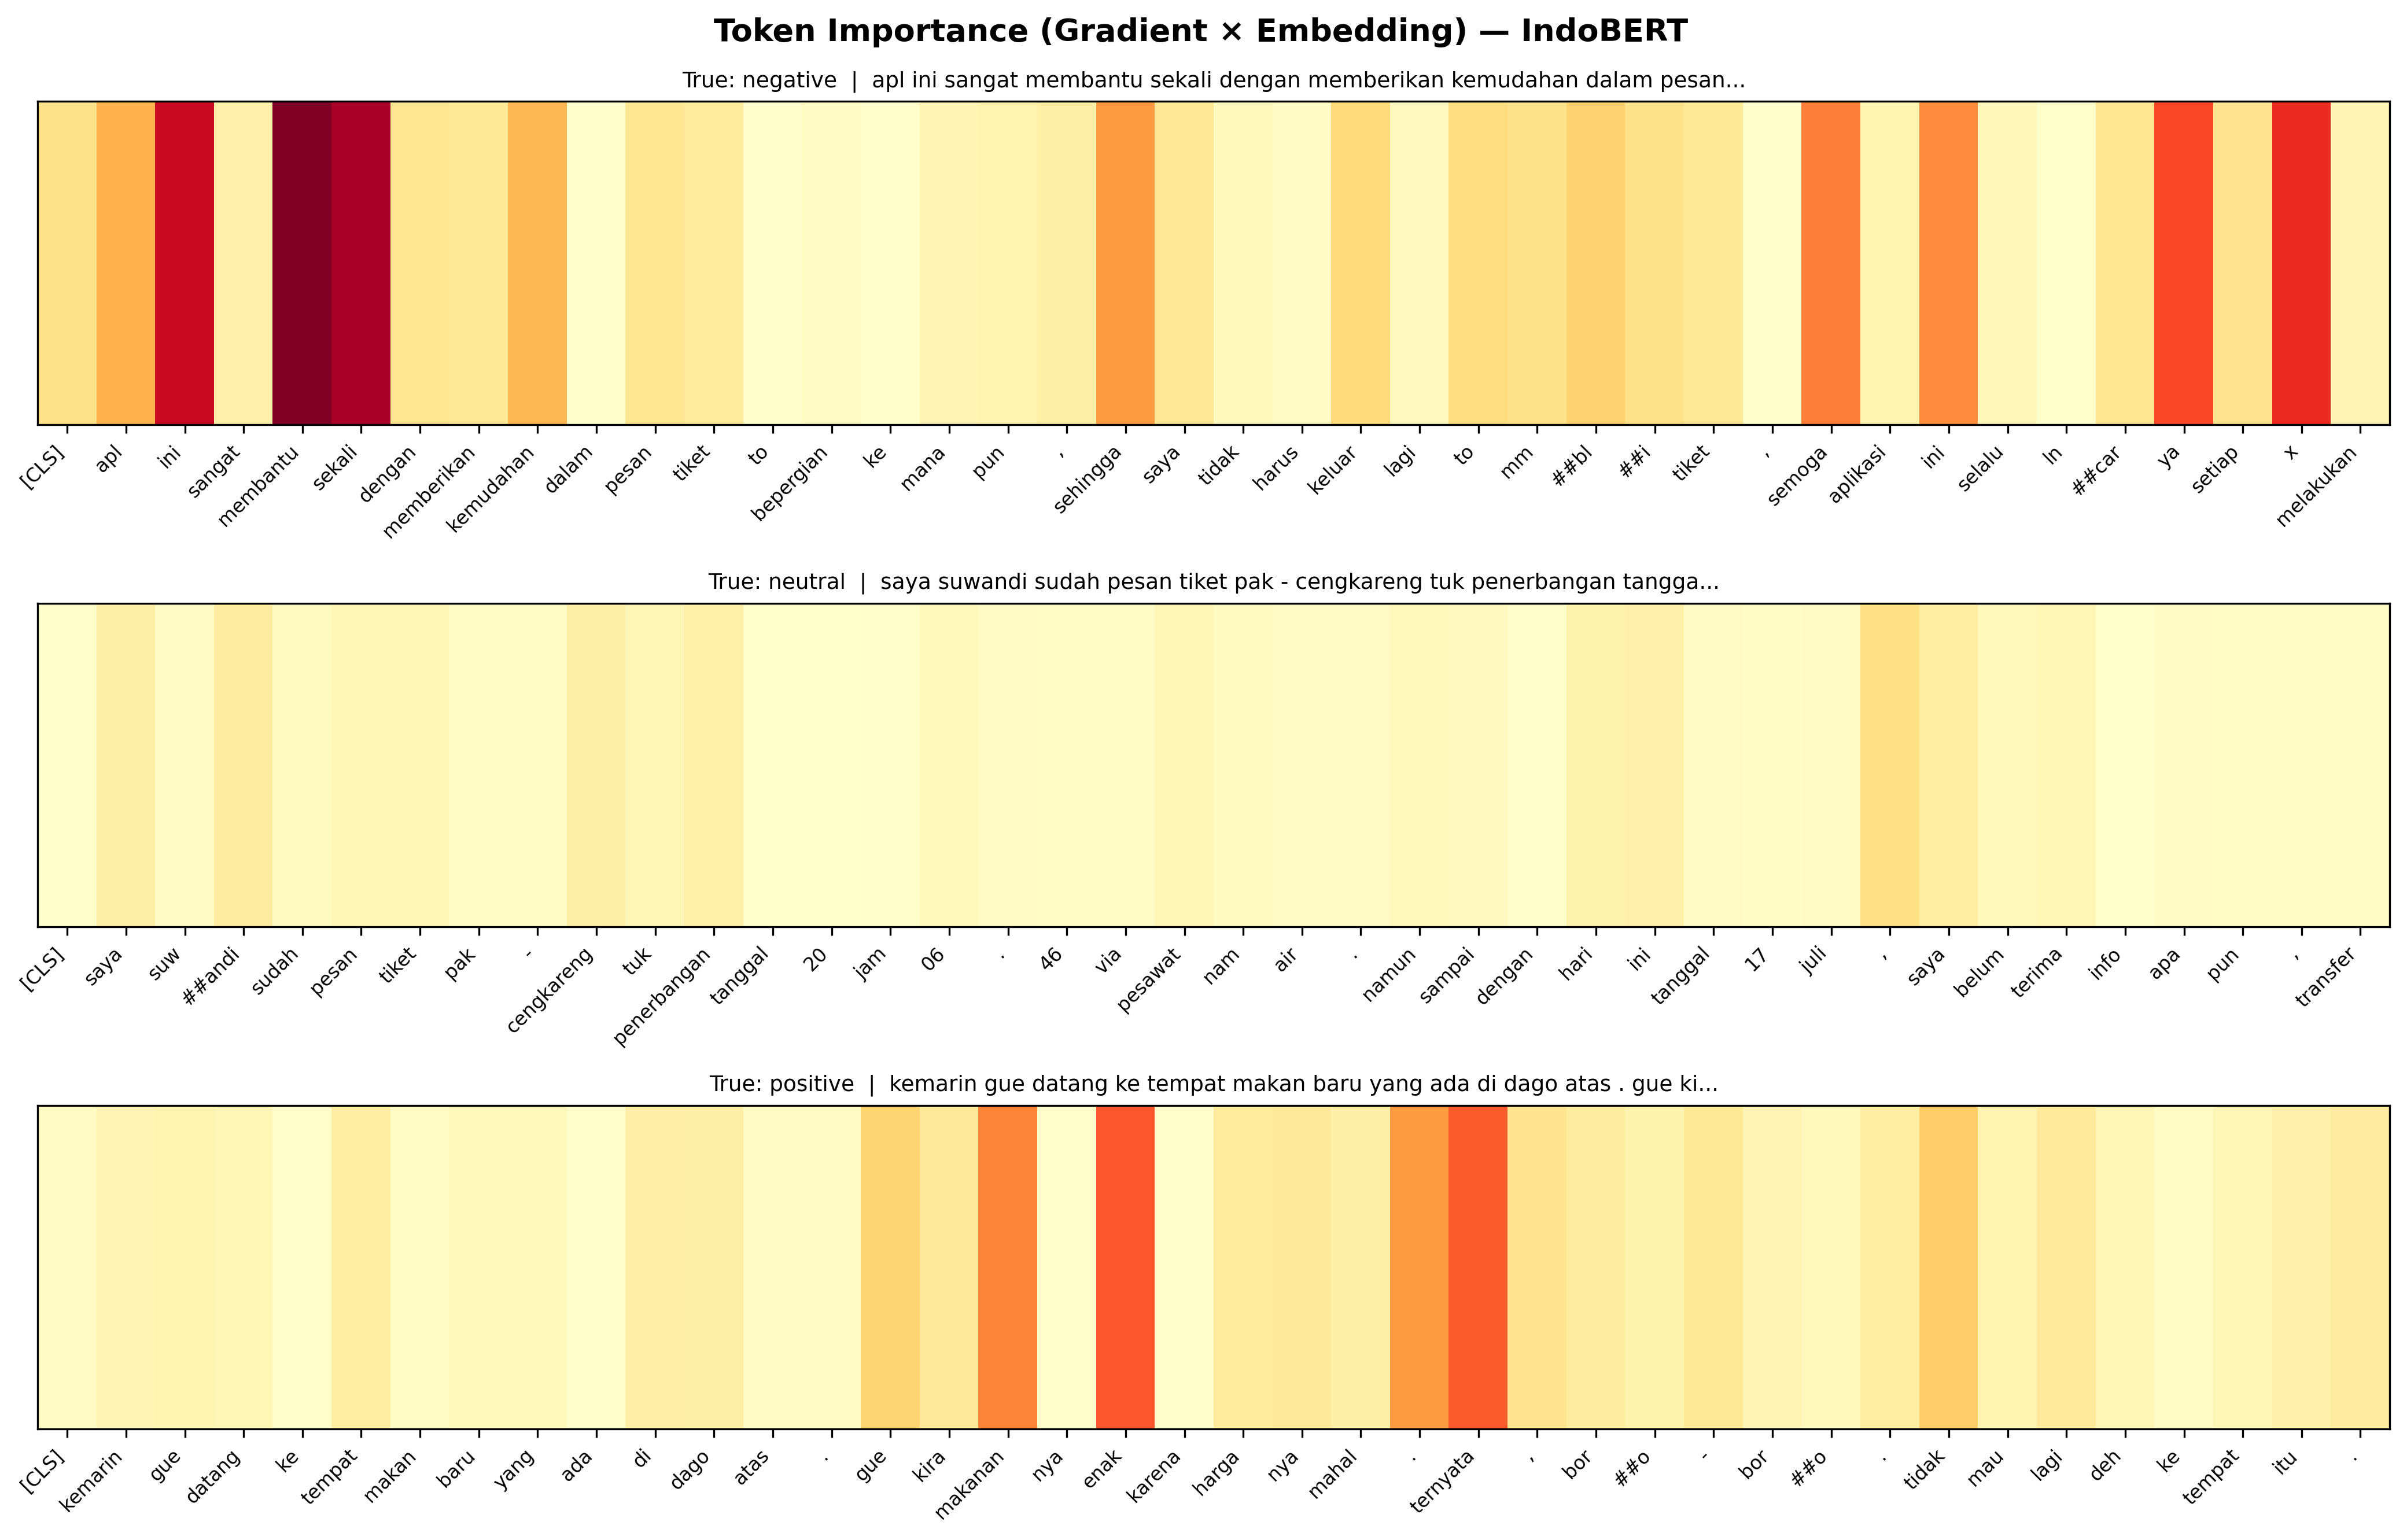
\includegraphics[width=\columnwidth]{outputs/figures/fig6_token_importance.png}}
\caption{Token-level attribution.}
\label{fig:token_importance}
\end{figure}

\subsection{Efficiency Analysis}

Table~\ref{tab:efficiency} and Fig.~\ref{fig:efficiency_tradeoff} show the efficiency profile. IndoBERTweet dominates the Pareto frontier: best F1 (0.9015) at 8.21\,ms/sample and 1,312\,MB GPU memory. The full ensemble doubles both latency and memory while yielding 7.16 fewer F1-Macro points, making it strictly Pareto-dominated. The SVM offers a no-GPU fallback at 0.741 F1 and near-zero latency.

\begin{table}[htbp]
\caption{Efficiency Analysis on NVIDIA T4 GPU}
\label{tab:efficiency}
\begin{center}
\begin{tabular}{lrrrr}
\toprule
\textbf{Model} & \textbf{Params} & \textbf{Lat.(ms)} & \textbf{Mem.(MB)} & \textbf{F1} \\
\midrule
TF-IDF SVM    & 0.05M  & 0.008  & 0      & 0.741 \\
IndoBERT      & 124.4M & 8.04   & 1,312  & 0.894 \\
IndoBERTweet  & 110.6M & 8.21   & 1,312  & \textbf{0.902} \\
Full Ensemble & 235.1M & 16.26  & 2,624  & 0.830 \\
\bottomrule
\end{tabular}
\end{center}
\end{table}

\begin{figure}[htbp]
\centerline{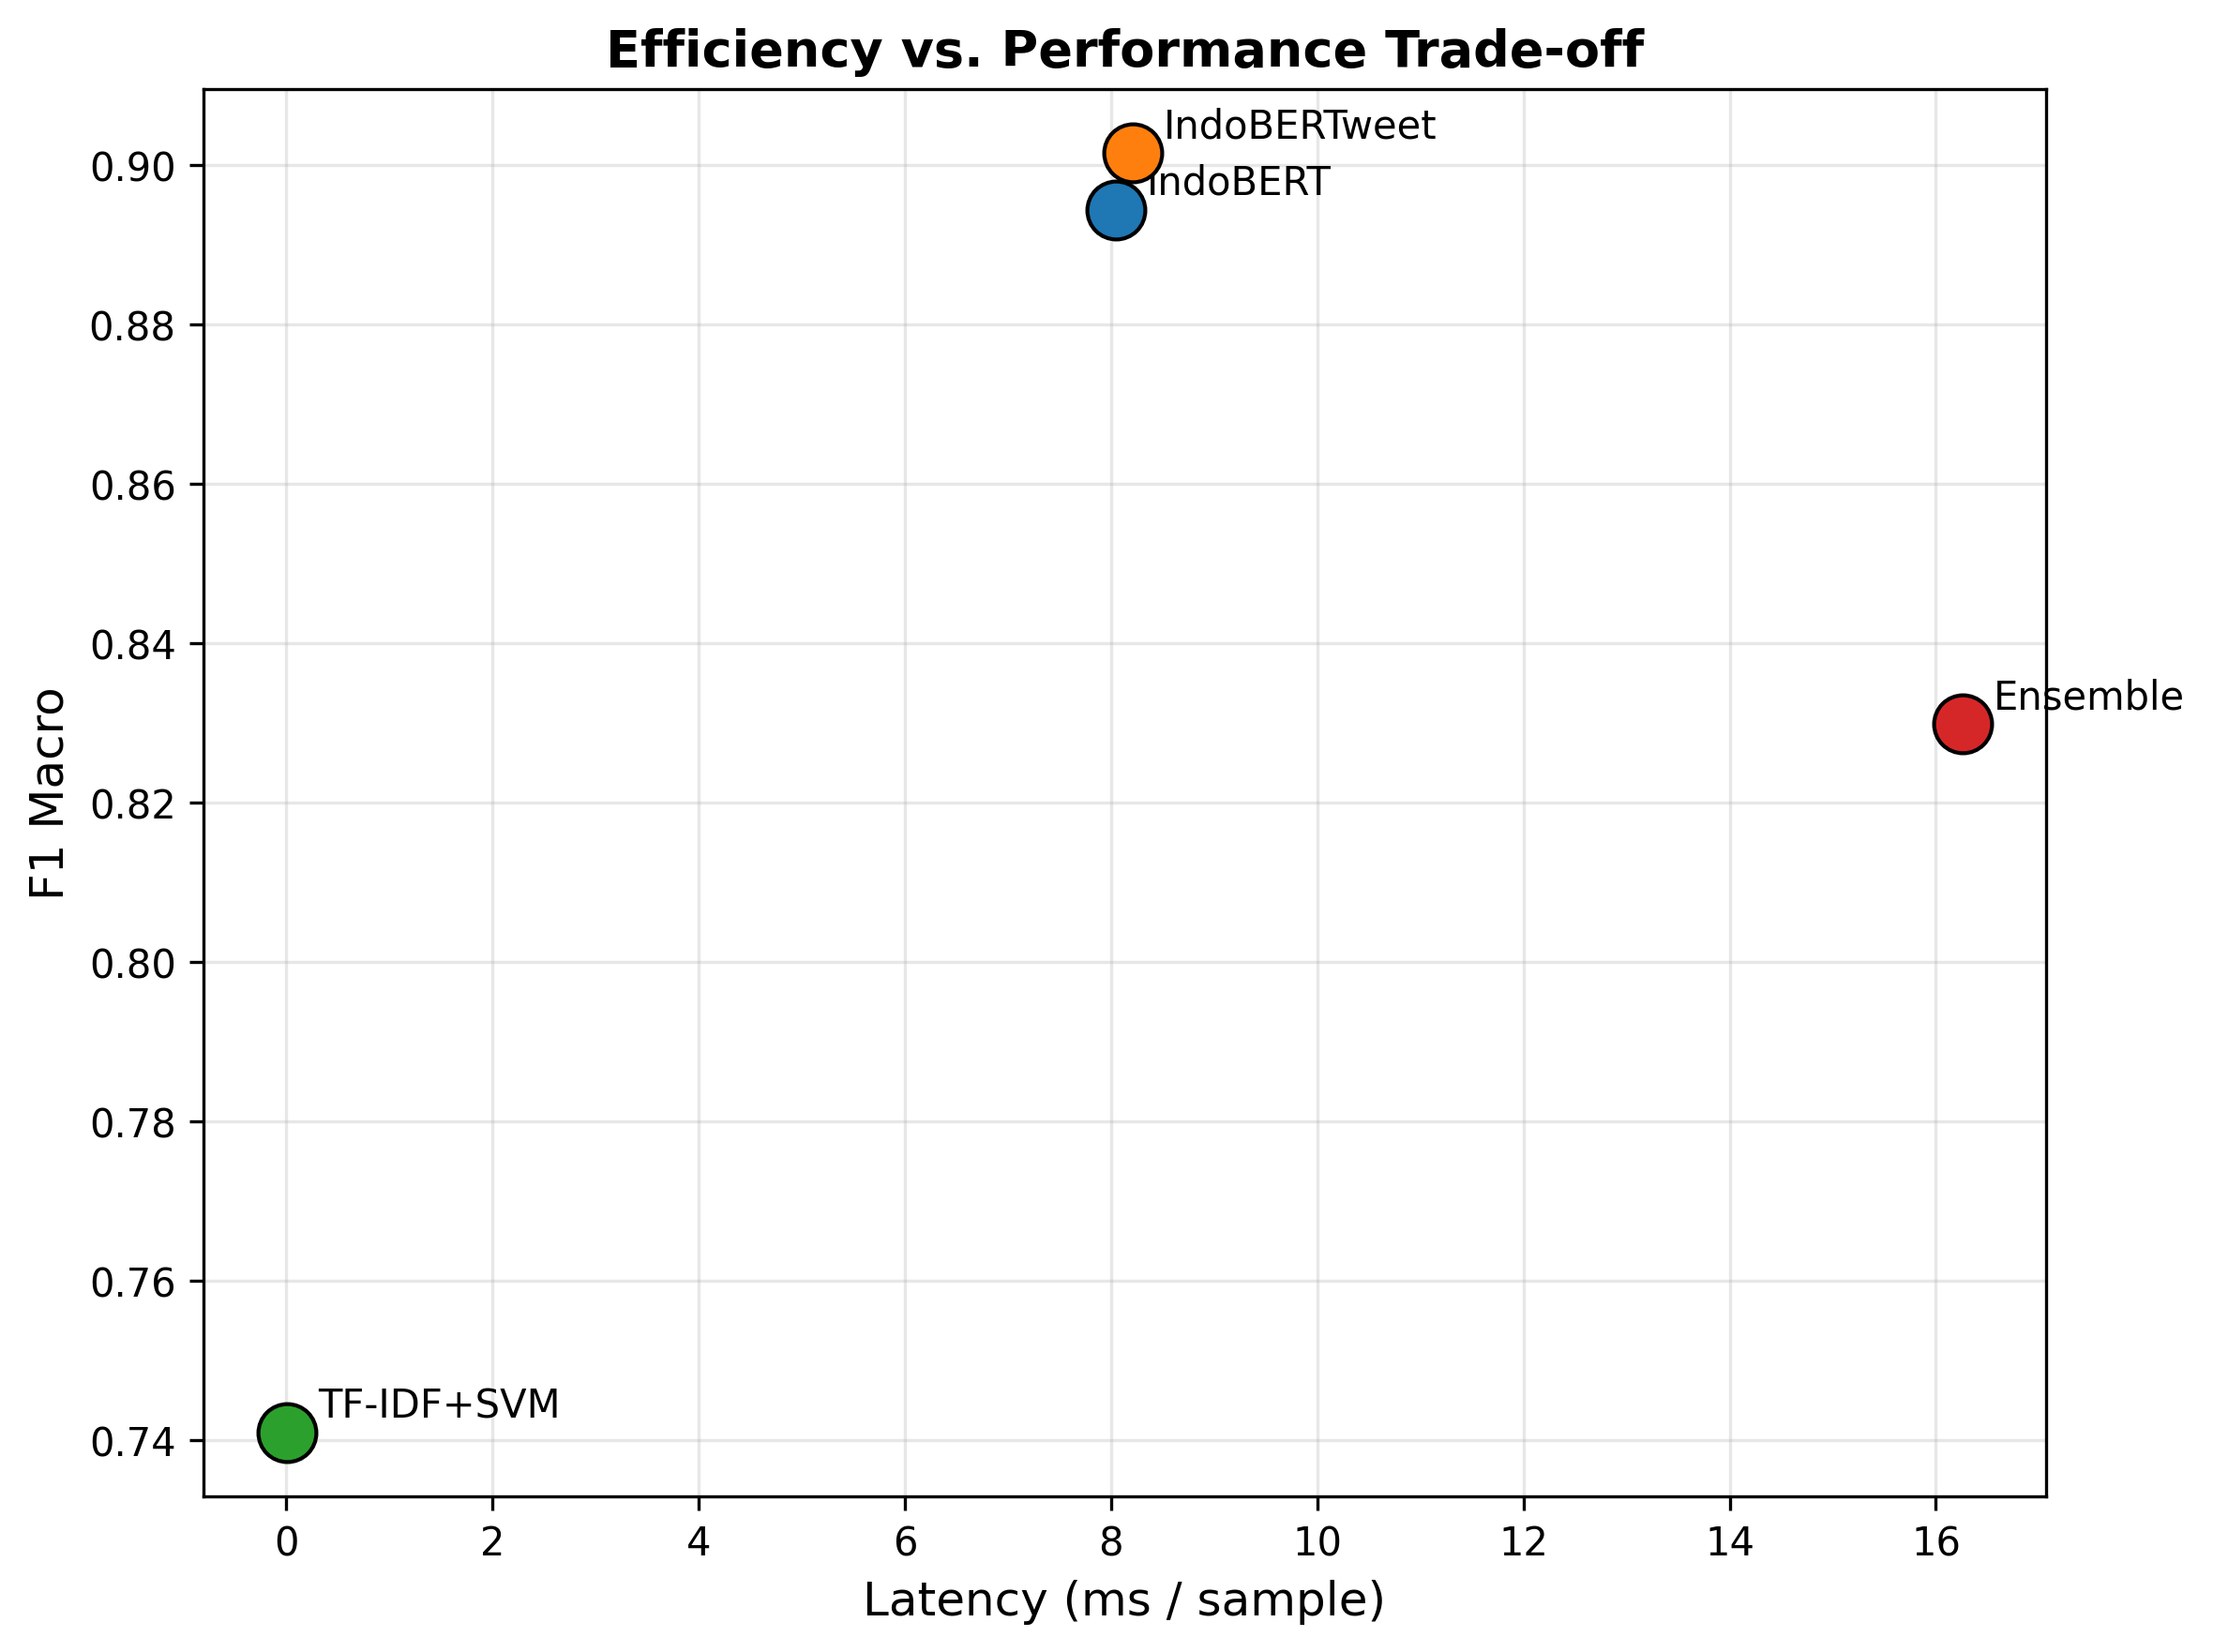
\includegraphics[width=\columnwidth]{outputs/figures/fig7_efficiency_vs_performance.png}}
\caption{Performance-efficiency tradeoff.}
\label{fig:efficiency_tradeoff}
\end{figure}

\subsection{Failure Case Analysis}

Inspection of 61 misclassified test samples reveals three patterns. \textbf{Sarcasm:} tweets like \textit{``iya enak banget soal nya''} (``oh yeah, that's so great,'' ground truth: negative) are predicted positive because the surface token carries positive valence. SHAP also confirms SVM\_pos receives highest attribution, as TF-IDF cannot encode discourse context \cite{b24}. \textbf{Neutral boundary confusion:} factual product statements and informative tweets were systematically misclassified as positive or negative. Moreover, the ensemble's neutral F1 score of 0.6438 was the most acute symptom of training imbalance exacerbated by SVM dominance. \textbf{Code-mixed text:} multi-token phrases combining English adjectives with Indonesian grammar produce inconsistent predictions even in IndoBERTweet, highlighting the persistent pre-training coverage gap.

Instance-level SHAP analysis of individual misclassified samples provides actionable diagnostic depth. For example, the sarcastic inputs, SVM\_pos receives attribution 2--4$\times$ larger than IndoBERTweet\_neg, even when IndoBERTweet assigns correct high negative probability. The very high confidence of SVM overrides the nuanced signals from transformers at the meta-learner level. This instance-level pattern suggests a practical mitigation: predictions where the SVM's aggregate SHAP magnitude exceeds the combined transformer SHAP magnitude can be flagged for human review, enabling a selective confidence-based routing strategy that decouples high-uncertainty ensemble decisions from fully automated deployment without requiring retraining.

% ============================================================
\section{Conclusion}
% ============================================================

This paper demonstrated that a heterogeneous stacking ensemble of IndoBERT, IndoBERTweet, and TF-IDF SVM underperforms IndoBERTweet alone by 7.16 F1-Macro points on the IndoNLU SmSA benchmark. SHAP analysis of the Logistic Regression meta-learner reveals the cause: Platt-scaled SVM probabilities dominate attribution (60.3\%) by producing extreme confidence values that override the smoother transformer outputs, a meta-learner calibration failure invisible without post-hoc interpretability. Ablations confirm SVM removal recovers 6.46 points. For deployment, IndoBERTweet fine-tuned individually is the dominant choice: best F1 at standard transformer overhead with no ensemble infrastructure.

\textbf{Limitations.} Experiments are on a single benchmark and generalization to other Indonesian domains (e-commerce, reviews, news) is untested. We diagnosed calibration problems but did not implement fixes (for example, temperature scaling) \cite{b18}. Because, this is intentionally left as direct future work to maintain the paper's diagnostic focus. Additionally, a slang dictionary published in 2018 may not cover the ever-evolving informal vocabulary, and regular lexicon updates would improve the coverage of SVM preprocessing \cite{b15}. The results were obtained from a single random seed, but the variance between seeds would strengthen the statistical claim.

\textbf{Future work.} The scarcity of neutral classes must be addressed through balanced sampling across classes or data augmentation, and evaluating calibration-corrected stacking. Specifically, applying temperature scaling, by dividing the logit of each model by a scalar learned before softmax, will normalize the probability scale across the model family and is the most direct fix for the failures identified here \cite{b18}. Isotonic regression offers a non-parametric alternative when the calibration curve is non-monotonic. An ensemble fusion method that operates on class ranks rather than probability quantities (e.g., Borda count aggregation) completely ignore calibration compatibility and require further investigation. Extending the SHAP-based diagnostic framework to aspect-level and multi-label Indonesian language tasks will test whether calibration mismatches exhibit similar patterns as the complexity of the output space increases. Improvements that account for sarcasm and cross-language transfer for code-mixed input are still an undeveloped direction \cite{b24}.

% ============================================================
\begin{thebibliography}{00}

\bibitem{b1} W. Kemp, ``Digital 2024: Indonesia,'' DataReportal, Jan. 2024.

\bibitem{b2} F. Koto, A. Rahimi, J. H. Lau, and T. Baldwin, ``IndoLEM and IndoBERT: A benchmark dataset and pre-trained language model for Indonesian NLP,'' in \textit{Proc. COLING}, 2020, pp. 757--770.

\bibitem{b3} B. Wilie et al., ``IndoNLU: Benchmark and resources for evaluating Indonesian natural language understanding,'' in \textit{Proc. AACL}, 2020, pp. 843--857.

\bibitem{b4} F. Koto, J. H. Lau, and T. Baldwin, ``IndoBERTweet: A pre-trained language model for Indonesian Twitter,'' in \textit{Proc. EMNLP}, 2021, pp. 10762--10776.

\bibitem{b5} R. Sinaga and M. L. Khodra, ``Aspect-based sentiment analysis for Indonesian tourism reviews,'' in \textit{Proc. ICAICTA}, 2019.

\bibitem{b6} A. Imanuel, H. Sungkono, and A. Chowanda, ``Indonesian aspect-based sentiment analysis using BiLSTM and BERT,'' \textit{Procedia Computer Science}, vol. 216, pp. 476--483, 2023.

\bibitem{b7} D. H. Wolpert, ``Stacked generalization,'' \textit{Neural Networks}, vol. 5, no. 2, pp. 241--259, 1992.

\bibitem{b8} A. Khan, U. Naseer, A. M. Khattak, and S. U. Khan, ``RRLS: A stacked ensemble model for Urdu sentiment analysis,'' \textit{Scientific Reports}, vol. 15, no. 1, 2025.

\bibitem{b9} M. Younas et al., ``RoBERTa-BiLSTM: A hybrid deep learning model for sentiment analysis,'' arXiv:2406.00367, 2024.

\bibitem{b10} M. S. Sivri, ``Combining sentiment analysis models using stacking ensemble on BIST30 stocks,'' \textit{J. Hendese}, vol. 1, no. 2, pp. 91--97, 2024.

\bibitem{b11} S. M. Lundberg and S.-I. Lee, ``A unified approach to interpreting model predictions,'' in \textit{NeurIPS 30}, 2017, pp. 4765--4774.

\bibitem{b12} C. Sun, L. Huang, and X. Qiu, ``Utilizing BERT for aspect-based sentiment analysis via constructing auxiliary sentence,'' in \textit{Proc. NAACL}, 2019, pp. 380--385.

\bibitem{b13} J. Vig, ``A multiscale visualization of attention in the transformer model,'' in \textit{Proc. ACL System Demonstrations}, 2019, pp. 37--42.

\bibitem{b14} B. Wilie et al., ``IndoNLU benchmark,'' GitHub, 2020. [Online]. Available: https://github.com/indobenchmark/indonlu

\bibitem{b15} A. Salsabila, Y. Winatmoko, N. Septiandri, and A. Jamal, ``Colloquial Indonesian lexicon,'' in \textit{Proc. IALP}, 2018, pp. 237--241.

\bibitem{b16} J. Devlin, M.-W. Chang, K. Lee, and K. Toutanova, ``BERT: Pre-training of deep bidirectional transformers,'' in \textit{Proc. NAACL}, 2019, pp. 4171--4186.

\bibitem{b17} M. T. Ribeiro, S. Singh, and C. Guestrin, ```Why should I trust you?': Explaining any classifier,'' in \textit{Proc. KDD}, 2016, pp. 1135--1144.

\bibitem{b18} C. Guo, G. Pleiss, Y. Sun, and K. Q. Weinberger, ``On calibration of modern neural networks,'' in \textit{Proc. ICML}, 2017, pp. 1321--1330.

\bibitem{b19} S. Desai and G. Durrett, ``Calibration of pre-trained transformers,'' in \textit{Proc. EMNLP}, 2020, pp. 295--302.

\bibitem{b20} B. Lakshminarayanan, A. Pritzel, and C. Blundell, ``Simple and scalable predictive uncertainty estimation using deep ensembles,'' in \textit{NeurIPS 30}, 2017, pp. 6402--6413.

\bibitem{b21} M. Minderer et al., ``Revisiting the calibration of modern neural networks,'' in \textit{NeurIPS 34}, 2021, pp. 15682--15694.

\bibitem{b22} S. Cahyawijaya et al., ``NusaCrowd: Open source initiative for Indonesian NLP resources,'' in \textit{Findings of ACL}, 2023, pp. 13745--13818.

\bibitem{b23} P. Atanasova, J. G. Simonsen, C. Lioma, and I. Augenstein, ``A diagnostic study of explainability techniques for text classification,'' in \textit{Proc. EMNLP}, 2020, pp. 3256--3274.

\bibitem{b24} S. Oprea and W. Magdy, ``iSarcasm: A dataset of intended sarcasm,'' in \textit{Proc. ACL}, 2020, pp. 1279--1289.

\end{thebibliography}

\end{document}
